% !TEX root = main.tex

\section{Results \label{sec:5_results}}
While it is the global characteristic sequence that is most relevant to the closure relations this work has set out to evaluate, it is nonetheless instructive to see the shape of the global distributions themselves. We would like to remind the reader that these distributions do not hold at every local point in the crystal--the local distributions are poorly behaved due to the discrete nature of the segments--they do describe the average strength of orientation fluctuations in the crystal. Let us turn, then, our attention to these global distributions, shown in \cref{fig:Distributions}. It is noted that there is a sharp peak at zero fluctuation (\cref{fig:Distributions}a), corresponding to the local regions being pierced only by a single dislocation. In these cases, the local fluctuation distribution is a Dirac mass at zero fluctuation. The strength of this peak in the global distribution can be thought of as the density-weighted fraction of such regions in the crystal. The remaining distribution at non-zero fluctuations (\cref{fig:Distributions}b), is closer in shape to a Cauchy distribution than to a von Mises distribution. The general trend---as can be seen from \cref{fig:Distributions}---is that short coarse-graining lengths correspond to narrow distributions about zero fluctuation, and long coarse-graining lengths to broad distributions.

\begin{figure}
    \centering
    \subfloat{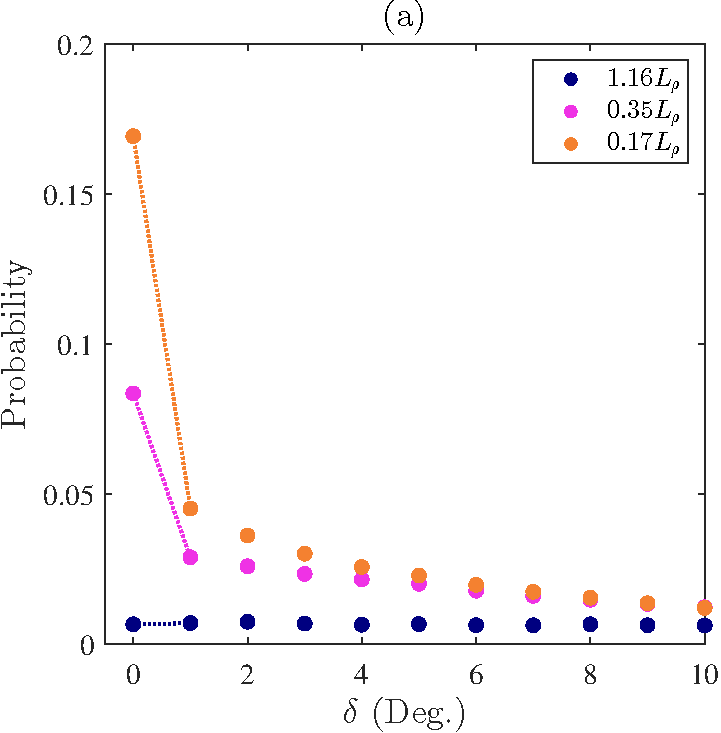
\includegraphics[height=2.5in]{Images/fig2a.pdf}}\\
    \subfloat{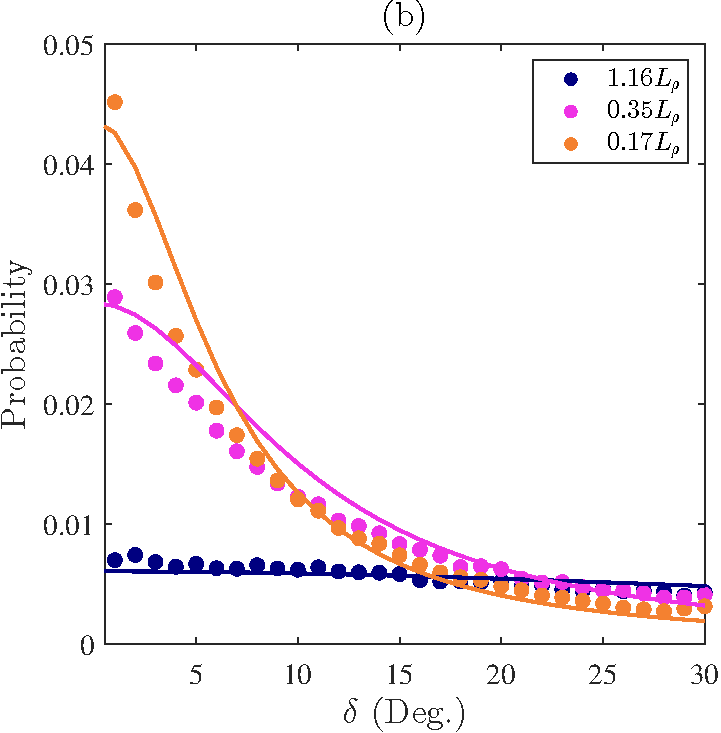
\includegraphics[height=2.5in]{Images/fig2b.pdf}}
    \caption{Typical global orientation fluctuation distributions from the dataset. Both figures show a selection of the orientation fluctuation distribution functions at various coarse-graining lengths. Fig. 2a shows the sharp peak at zero fluctuation angle coming from single-crossing events, and Fig. 2b shows the same functions with the zero fluctuation point shielded from view. Cauchy fits are shown on the latter figure to demonstrate the shape of the distributions at non-zero fluctuation angle.}
    \label{fig:Distributions}
\end{figure}
The trend of coarse-graining leading to distribution broadening can be seen explicitly by fitting the discrete distributions of \cref{fig:Distributions} to an analytical form. The form chosen is:
\begin{equation}
    f(\delta) = P_0 \hat{\delta}(\delta) + (1-P_0) C(\delta\vert\gamma)
\end{equation}
where $C(\delta\vert\gamma)$ is the wrapped Cauchy distribution (\cite{mardiaStatisticsDirectionalData1975}):
\begin{equation}
    C(\delta\vert\gamma) = \frac{1}{2\pi} \frac{\sinh \gamma}{\cosh \gamma - \cos \delta}
\end{equation}
The parameters--the null probability $P_0$ and Cauchy parameter $\gamma$--were obtained by fitting a wrapped Cauchy distribution to the obtained global distributions while omitting the zero fluctuation data point. The results of this fitting process for various coarse-graining lengths are shown in \cref{fig:distributionfits}. In \cref{fig:distributionfits}a, we see the disappearance of the null probability as we move to longer coarse-graining lengths approaching the mean dislocation spacing. This corresponds to a decreased likelihood of single-piercing events as local coarse-graining volumes grow. Similarly, we see in \cref{fig:distributionfits}b the growth of the full-width-at-half-maximum (twice the Cauchy parameter $\gamma$ of the distribution, ranging from only a few degrees for fine scales up to almost a quarter of the unit circle for scales approaching the mean dislocation spacing. This broadening of the distribution indicates the allowance of progressively stronger orientation fluctuations as the coarse-graining process considers larger representative volumes.
\begin{figure}
    \centering
    \subfloat{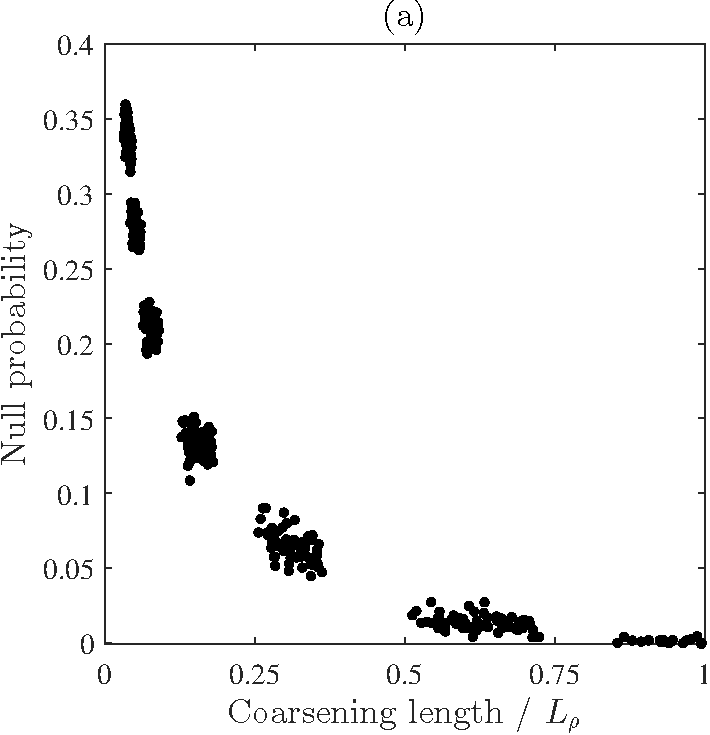
\includegraphics[height=2.5in]{Images/fig3a.pdf}}\\
    \subfloat{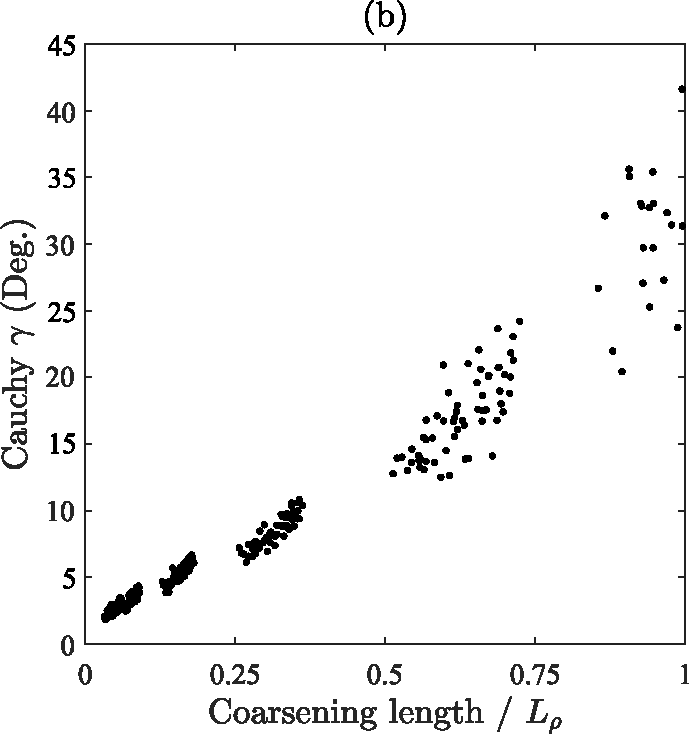
\includegraphics[height=2.5in]{Images/fig3b.pdf}}
    \caption{Trend of distributions with coarse-graining length. The two parameters chosen to describe the shape of the distributions are shown as coarse-graining length is increased: Dirac mass weight at zero fluctuation--the prevalence of zero crossing events--is shown in (a) while the Cauchy parameter--the half-width-at-half-maximum--is shown in (b).}
    \label{fig:distributionfits}
\end{figure}

We may now turn our attention to the characteristic sequences which are the focus of the present work. \Cref{fig:characteristicsequence} shows the first three components in the characteristic sequence for various coarse-graining lengths. Recalling that a perfect Dirac distribution at zero fluctuation has a characteristic sequence everywhere equal to unity, it should not surprise that the fine coarse-graining lengths correspond to near-unit characteristic sequences. As we move to coarser scales, the polarization ($\beta_1$, shown in \cref{fig:characteristicsequence}a) decays. The higher-order components $\beta_2, \ \beta_3$---shown in \cref{fig:characteristicsequence}b-c, respectively---decay more rapidly than the polarization. 

\begin{figure*}
    \centering
    \subfloat{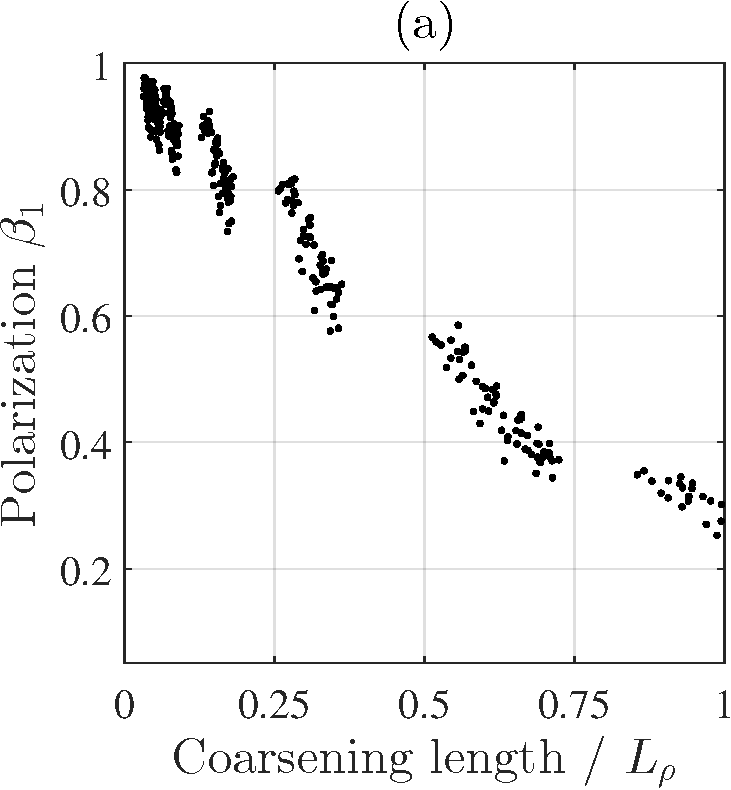
\includegraphics[height=2.2in]{Images/fig4a.pdf}}\hspace{\fill}
    \subfloat{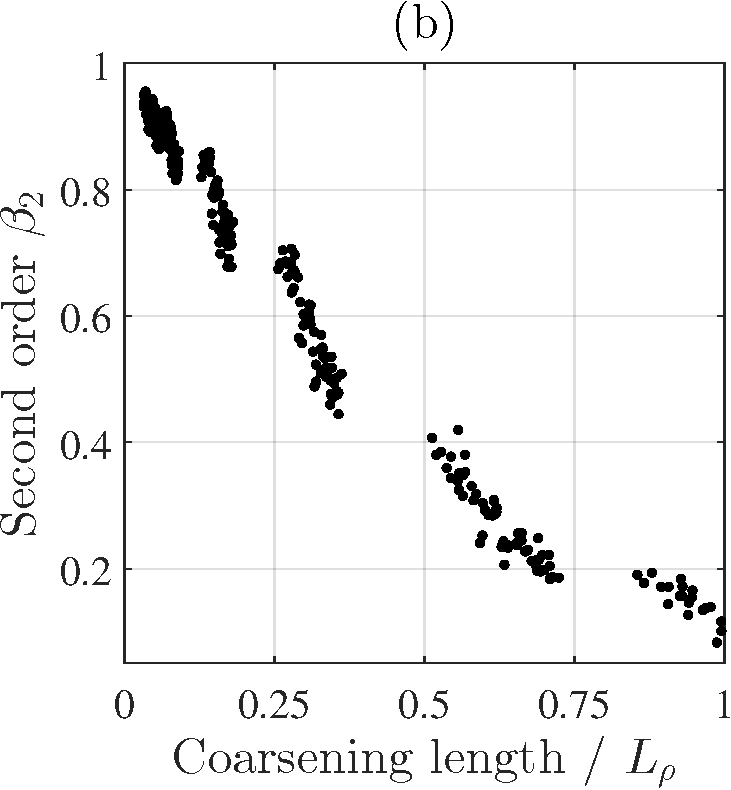
\includegraphics[height=2.2in]{Images/fig4b.pdf}}\hspace{\fill}
    \subfloat{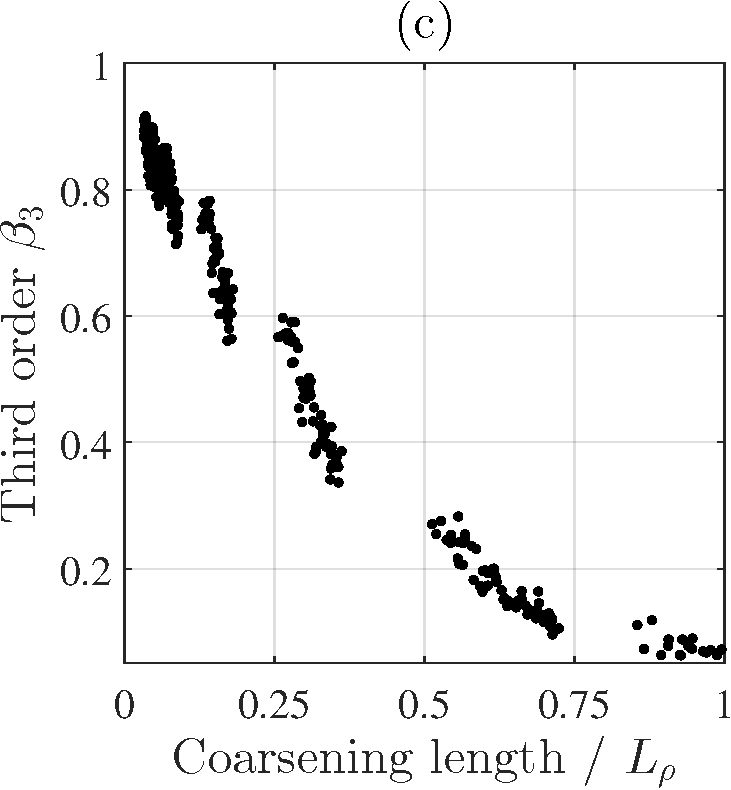
\includegraphics[height=2.2in]{Images/fig4c.pdf}}
    \caption{Characteristic sequence components. The first- (a), second- (b), and third-order (c) characteristic components are plotted against coarse-graining length.}
    \label{fig:characteristicsequence}
\end{figure*}

The main question of the present work, however, is how well the closure approximations reproduce the higher-order components. \Cref{fig:closure} shows relative error (approximation/true value) of the line bundle and maximum entropy closure approximations across scales. The line bundle and maximum entropy approximations of the second order component are given by
\begin{align}
    \beta_2^{(\mathrm{LB})} &= \beta_1 ^2 \\
    \beta_2^{(\mathrm{ME})} &= \frac{1}{2}(\beta_1^2+\beta_1^6)
\end{align}
and the third order component by
\begin{align}
    \beta_3^{(\mathrm{LB})} &= \beta_1\beta_2 \\
    \beta_3^{(\mathrm{ME})} &= 2\sqrt{2}\beta_1(\sqrt{1+\beta_2} -3)
\end{align}
\Cref{fig:closure}a shows the relative error in the approximations to the second component of the fluctuation distribution utilized in closing the evolution hierarchy at first order. It is seen that the line bundle closure closely approximates the second order component of the distribution for coarse-graining lengths shorter than half of the mean dislocation spacing. The approximation shows significant variance but still decent agreement with the true second order component for scales up to three-quarters of the mean spacing. The maximum entropy approximation to the second order component, however, performs poorly for all but the finest of coarse-graining lengths, consistently underpredicting the magnitude of the second order component. This is due to the rapid decay of the $\beta_1^6$ term which is simply not present in the ground truth data. {This favoring of the line bundle (wrapped Cauchy-like) over the maximum entropy (assuming von  Mises distribution at first order) first order closure is consistent with the Cauchy rather than von Mises shape of the observed fluctuation distribution functions (cf. \cref{fig:Distributions}b).}
\begin{figure*}
    \centering
    \subfloat{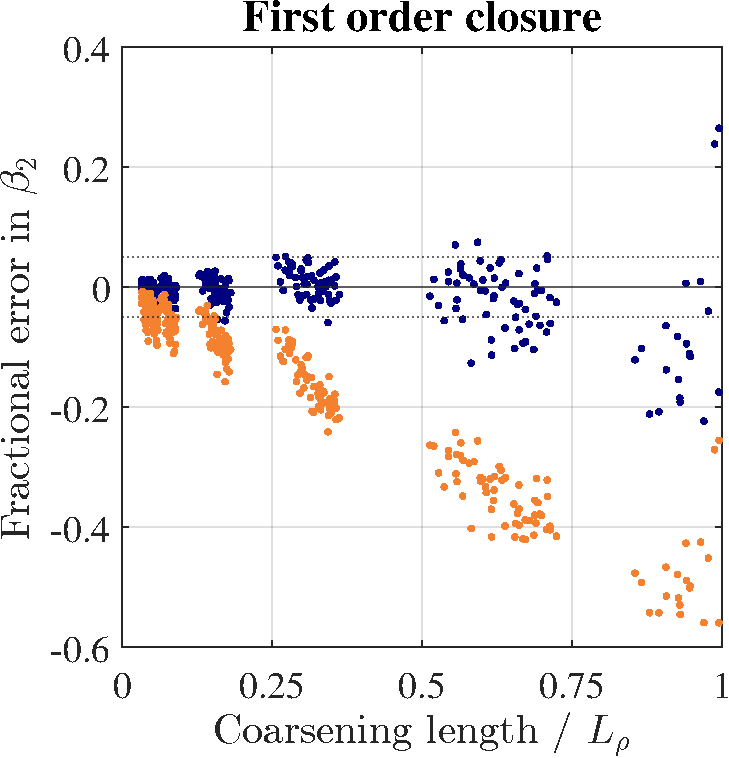
\includegraphics[height=2.5in]{Images/fig5a.pdf}}\hspace{.5in}
    \subfloat{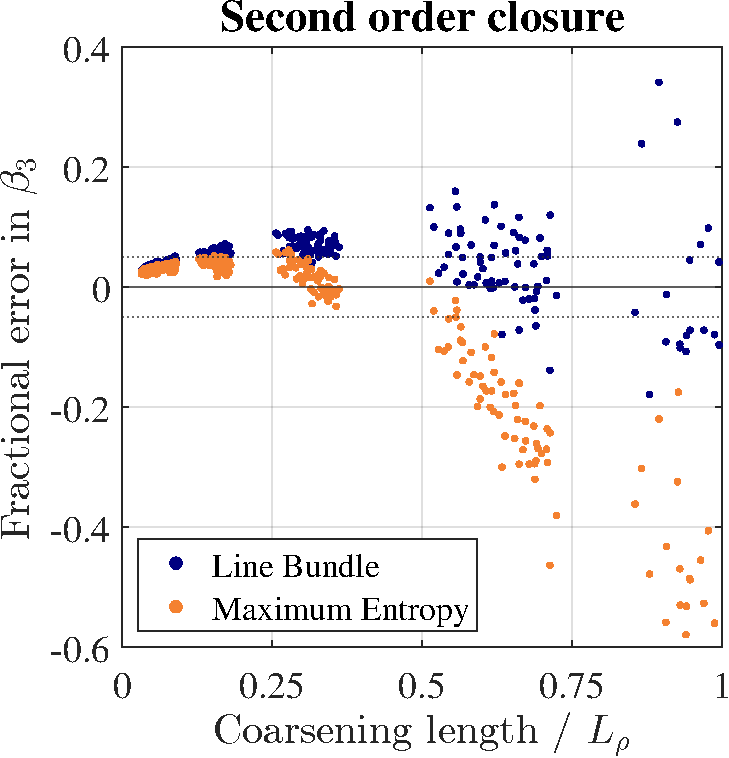
\includegraphics[height=2.5in]{Images/fig5b.pdf}}
    \caption{Fractional closure errors associated with the line bundle and maximum entropy closure forms. These show the fractional error in closing the orientation description at first order (approximating $\beta_2$ as a function of $\beta_1$) and at second order (approximating $\beta_3$ as a function of $\beta_1,\beta_2$) as a function of course graining length.}
    \label{fig:closure}
\end{figure*}

The relative errors for approximations to the third order component of the distribution (second order closure) are shown in \cref{fig:closure}b. At this order, both approximations perform well for coarse-graining lengths shorter than half the mean dislocation spacing. For longer lengths, the line bundle approximation remains a decent description of the third order component, although with the introduction of significant variance. The maximum entropy approximation, on the other hand, quickly begins to deviate from the ground truth for scales above half the dislocation spacing.